\documentclass[journal]{IAENGtran}

\ifCLASSINFOpdf
   \usepackage[pdftex]{graphicx}
   \DeclareGraphicsExtensions{.pdf,.jpeg,.png}
\else
   \usepackage[dvips]{graphicx}
   \DeclareGraphicsExtensions{.eps}
\fi

\begin{document}
\title{An Explanation Method of Unfamiliar Tourist Spots based on Roles of User's Familiar Spots}
\author{Kenta~Han and Daisuke~Kitayama

\thanks{K. T. Han is with the Graduate School of Engineering, Kogakuin University, Japan; e-mail: em18011@ns.kogakuin.ac.jp.}% <-this % stops a space
\thanks{D. Kitayama is with the Faculty of Informatics, Kogakuin University, Japan;  e-mail: kitayama@cc.kogakuin.ac.jp.}}% <-this % stops a space
\maketitle

\pagestyle{empty}
\thispagestyle{empty}

\begin{abstract}
In recent years, when user plans to travel, users often use tourist information on the Web.
However, travel often goes to an unfamiliar area, therefore it is difficult to get the tourist information properly.
Therefore, in order to support understanding of users' unfamiliar spots, we propose a method to explain tourist spots of unfamiliar area using tourist spots that have visited by users.
In this paper, at first, we generate the feature vector using user reviews of the tourist spot.
Next, we use the relative feature vector compared with already visited spots to extract the role of the tourist spot for the user.
Finally, we associate the visited spot with the unfamiliar spot by the similarity of the relative feature vector, and further extract keywords that explain the relation.
We also develop the prototype system, and we evaluate the effect of the explanatory information between the familiar spot and the unfamiliar spot.
\end{abstract}

\begin{IAENGkeywords}
tourist spots, explainability, user reviews, paragraph vector
\end{IAENGkeywords}

\IAENGpeerreviewmaketitle

\section{Introduction}
\label{sec:Introduction}
\IAENGPARstart{W}{hen} deciding the travel destination, the traveler selects tourist spots by planning a travel, browsing web pages of tourist spots and tourist guidebooks.
However, travel often goes to an unfamiliar area, therefore it is difficult to get the tourist information properly.
At this time, it is considered that the user often decides the tourist spot by looking at the ranking and recommendation information of the tourist spot search engine.
In a tourist spot search engine such as Tripadvisor\footnote{https://www.tripadvisor.com/} and Jalan\footnote{Jalan is a review posting site on tourist spots in Japan. https://www.jalan.net/kankou/}, the user who visited there about a certain tourist spot posted reviews and there is a wealth of information on tourist spots.
However, since the user has no prior knowledge about the search area, what kind of tourist spot is to be confirmed one by one.
Therefore, in order to effectively understand various tourist spots, we think that it is effective if we compare an unfamiliar spot using a visited spot of user.
This is a kind of analogy that applies the matters that the user previously experienced to the current matter. In this case, the previous experience is the already visited spot and the current matter is the spot in the unfamiliar area.
For example, whereas unfamiliar spots such as ``Omotesando'' in Tokyo, Japan, if you explain that it is similar to the already visited ``Avenue des Champs-Elysees'' in Paris, it may make it easier to understand.

In this paper, in order to support understanding of users' unfamiliar spots, we propose a method to explain tourist spots of unfamiliar area using tourist spots that have visited by users.
In our method, the user inputs already visited spots and unfamiliar area.
At this time, we generate the feature vector using user reviews of the tourist spot.
Next, we use the relative feature vector compared with already visited spots to extract the role of the tourist spot for the user.
Finally, we associate the visited spot with the unfamiliar spot by the similarity of the relative feature vector, and further extract keywords that explain the relation.
By this way, we aim to rise understandability of unfamiliar spots.
Fig. \ref{fig:Photo_Image} shows a concept of the proposed method.

The structure of this paper is as follows.
In section \ref{sec:Related Work}, we introduce related works.
In section \ref{sec:An Explainaton Method of Unfamiliar Tourist Spots}, we describe the proposed method.
In section \ref{sec:Evaluation Experiment}, we discuss evaluation experiments and its results.
In section \ref{sec:Conclusions and Future Work}, we describe conclusions of this paper and our future work.

\begin{figure}[t]
  \begin{center}
    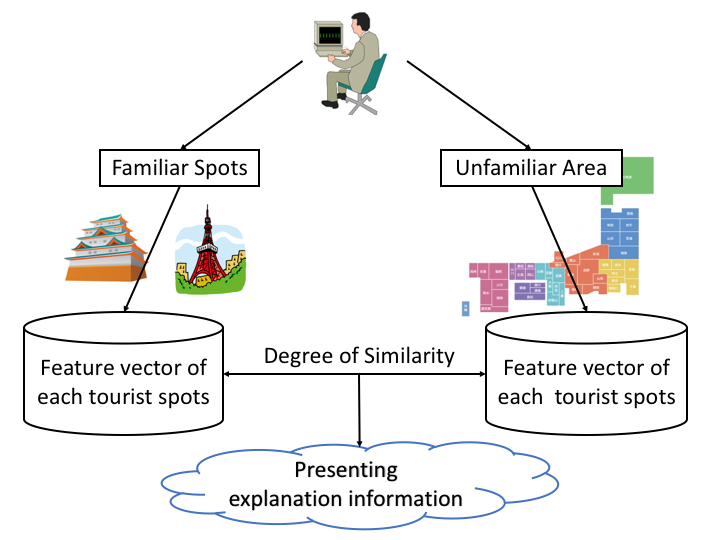
\includegraphics[clip,width=7.5cm,bb=0 0 720 540]{picture/Photo_Image_eng.png}
    \caption{An explanation method of unfamiliar tourist spots based on roles of user's familiar spots}
    \label{fig:Photo_Image}
   \end{center}
\end{figure}

\section{Related Work}
\label{sec:Related Work}
\subsection{Tourist spot retrieval and recommendation system}
\label{subsec:Tourist spot retrieval and recommendation system}

Many researches on retrieval and recommendation system using the user's experience history have been published.
Kurashima et al.\cite{Codd01} proposed a travel route recommendation method using geotag information of photos posted to Flickr as a travel history of people.
In this method, it is assumed that it is easy to move from a user's present location to a place easily accessible to the user's interest, and a behavior model is generated.
That geotagged photo aggregation of users can be regarded as personal travel history when sorted by time information, and we generate user behavior model using geotag information.
Kitamura et al.\cite{Codd02} proposed a method of recommending sightseeing spots based on estimating user's preferences of travel plan from past personal travel photographs using general object recognition.
Using an object recognition system to acquire keywords of subject information taken in the photos and represented the co-occurrence of the keywords by a graph visualization technique.
In addition, present a user interface that visualizes a graph with travel photos based on our graph visualization technique.
Cheng et al.\cite{Codd03} used photographs of freely available community contributions to focus on personalized trip recommendations, considering specific user profiles or attributes, suggested to consider personalized travel recommendations.

\subsection{The analogy and its applications}
\label{subsec:The analogy and its applications}
Analogies were pointed out as contributing to creative thinking\cite{Codd04}.
Analogical thinking works when acquiring a concept (called the target) from known knowledge (called the bases)\cite{Codd05}.
Many of the researches on analogy are given the base learning data and targeted problems, and the problems are solved by mapping the features of things to the feature of the problem\cite{Codd06}.
Gick et al. designed to investigate the use of analogies between disparate domains as a guide to finding solutions for an ill-defined problem.
Some studied about how to give learning data and functions\cite{Codd07}, and clarified whether to solve the problem depending on the degree of cognitive proficiency\cite{Codd08}.
In many of the conventional research including these, after giving bases and targets for analogy, we solve problems according to a certain procedure.
There are three types of structural similarities ``similarity of object level'' determined by the number of shared features, ``relationship similarity'' based on the degree of sharedness of relationships existing in the base and the relationship existing in the base, and similarity in the title solution or target level There is a certain ``pragmatic similarity''\cite{Codd05},\cite{Codd09}.

In the conventional method of using the user's experience history, many researches that analyze the geotag information of the history photograph and make it user's preference are performed.
In addition, it is well used in learning support on analogy technology.
In this research, using the review of familiar spots and unfamiliar spots, the relative features of each spot in each set of user familiar spot set and unfamiliar spot set are determined and associated, thereby supporting understanding of spots explanation information can be presented.
Moreover, because the quality of analogy is treated explicitly, it is considered to be similar to the similarity of structure "similarity of relationship level" by this research.

\section{An Explanation Method of Unfamiliar Tourist Spots}
\label{sec:An Explainaton Method of Unfamiliar Tourist Spots}
We propose an explanation method of unfamiliar tourist spots based on roles of user's familiar spots.
At first, the user inputs a set of tourist spots that have been visited and tourist area that user wishes to visit.
In our method, we generate the feature vector using user reviews of the tourist spot.
Next, we use the relative feature vector compared with already visited spots to extract the role of the tourist spot for the user.
Similarly, we calculate the relative feature vector of each tourist spot in the unfamiliar area by comparing with other tourist spots in that area.
Then, we associate the visited spot with the unfamiliar spot by the similarity of the relative feature vector.
Finally, we extract keywords that explain the relation.

\subsection{Generating feature vector using user reviews of spot}
\label{subsec:Generating feature vector using user reviews of spot}
In this paper, we will use the review data obtained from ``Jalan'' until the end of September 2016.
We generate feature vectors of tourist spots using paragraph vector\cite{Codd10}.
At this time, we combine all the reviews on a tourist spot and treat it as one document about the tourist spot.
In this paper, we use gensim\footnote{https://radimrehurek.com/gensim/models/doc2vec.html} that is a library of python for calculate paragraph vector.
We used Distributed Bag-of-Words as a learning method, and the number of dimensions was 300.
User reviews in Jalan are written by Japanese.
Therefore, we use MeCab\cite{Codd11} that is the Japanese morphological analyzer with dictionary ``mecab-ipadic-NEologd''\footnote{https://github.com/neologd/mecab-ipadic-neologd/}.

\subsection{Relative features for role of tourist spots}
\label{subsec:Relative features of tourist spots}

\begin{figure}[t]
  \begin{center}
    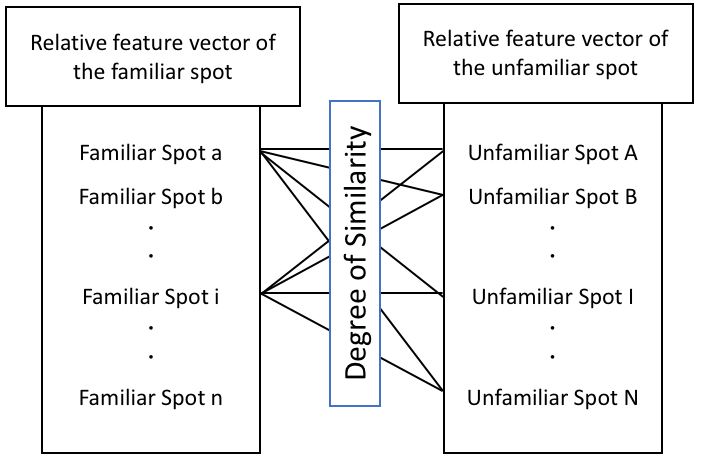
\includegraphics[clip,width=7.5cm,bb=0 0 720 540]{picture/Photo_CosSim_eng.png}
    % 類似度計算概念図
    \caption{Concept of similarity calculation}
    \label{fig:Photo_CosSim}
  \end{center}
\end{figure}

In our method, we extract the role of tourist spots by using the relative features of spots compared with other tourist spots.
We define the relative feature as the feature of the target spot when compared to the average feature of a set of tourist spots.
As an example, we consider the case where ``the Tokyo Metropolitan Government Building Observatories(TMGBO)'' and ``Kinkakuji Temple'' exist within the set of famous tourist spots in Japan.
At this time, relative features of ``Kinkakuji Temple'' is the temple, golden color, Kyoto, and so on.
On the other hand, relative features of ``TMGBO'' is the panoramic view, night view, building, Shinjuku, and so on.
When compared with various tourist spots, relative features tend to be general features, categories, places.

We will show other example.
We consider the case where there are ``Kinkakuji Temple'' and ``Kiyomizudera Temple'' in the set of temples in Kyoto, Japan.
At this time, the relative features of ``Kinkakuji Temple'' are gold color, gold leaf, brilliance, and so on.
On the other hand, the relative features of ``Kiyomizudera Temple'' are the stage, the panoramic view, and so on.
Because both are temples existing in Kyoto, features related to Kyoto and temples do not appear as relative features.
Instead, more detailed features are obtained as relative features.

The relative feature vector $r_{state,i}$ is defined as formula \ref{math:Vector difference}.
The relative feature vector is obtained by subtracting the average of feature vectors of other spots from its own feature vector.
\begin{equation}
  r_{state,i}=s_i-average(S_{state}-s_i)
  \label{math:Vector difference}
\end{equation}
Where, $S_{state} =\{s_1,s_2,\dots,s_n\}$ is a familiar spot set or an unfamiliar spot set.
When $state$ is $'f'$, it means familiar spot set.
When $state$ is $'u'$, it means unfamiliar spot set.
$s_i$ is a feature vector of a tourist spot in the set $S_{state}$.

\subsection{Determination of explainable spot}
\label{subsec:Determination of explainable spot}
We use a familiar spot as an explanation of the spot in an unfamiliar area.
Therefore, we associate unfamiliar spots and familiar spots with similarity that is calculated by the relative feature vector of the familiar spot $r_{f,i}$ and the unfamiliar spot $r_{u,j}$ (Fig. \ref{fig:Photo_CosSim} ).
For the similarity calculation, we use the cosine scale (formula \ref{math:CosSim}).
\begin{eqnarray}
  cos(r_{f,i},r_{u,j})=\frac{r_{f,i} \cdot r_{u,j}}{|r_{f,i}| \times |r_{u,j}|}
  \label{math:CosSim}
\end{eqnarray}

We explain the associating procedure.
First, we associate a spot with the highest degree of similarity to a certain spot.
At this time, if the similarity falls below the threshold (0.125 in this paper), we do not make association.
At this time, the result changes depending on whether the familiar spot having the highest degree of similarity to the unfamiliar spot is associated or the unfamiliar spot having the maximum similarity to the familiar spot is associated.

In the former the method, when all similarities exceed the threshold, all familiar spots have corresponding spots but not all unfamiliar spots have corresponding spots.
On the other hand, in latter method, when all similarities exceed the threshold, all unfamiliar spots have corresponding spots.
In our method, in order to give an explanation for unfamiliar spot, we adopt the latter method.

\subsection{Extraction of explainable words for role}
\label{subsec:Extraction of explainable words for role}
We present to users the keywords that represent the viewpoints of association between unfamiliar spots and familiar spots.
However, since we can not obtain the feature of a word from the relative feature vector, we extract words by another method.

As a premise, all reviews are divided into words by the Japanese morphological analyzer MeCab.
We use ``mecab-ipadic-NEologd'' as the dictionary as in Section \ref{subsec:Generating feature vector using user reviews of spot}.
However, the particle, auxiliary verb, adnominal, symbol, stop word are deleted.

We explain the procedure of keyword extraction. First, we obtain the feature word and tfidf value by the tfidf method from the target familiar spot and unfamiliar spot. Next, we calculate the harmonic mean of tfidf values as a score for feature words common to the two spots. Finally, we extract feature words with high scores as explainable words.

We calculate the feature value of a keyword in a spot is defined by the formula \ref{math:TFIDF}.
\begin{equation}
  TFIDF(t,d,state) = TF(t,d) \times log\Biggr(\frac{|S_{state}|}{DF(t,state)}\Biggr)
  \label{math:TFIDF}
\end{equation}
Where function $TF(t,d)$ returns the number of the keyword $t$ in the document $d$.
$d$ is a document combining all reviews of a spot into one.
Function $DF(t,state)$ retuns the number of documents that include keyword $t$.
$|S_{state}|$ is the total number of spots.
When $state$ is $f$, we calculate TFIDF value using a set of familiar spots that inputted by user.
When $state$ is $u$, we calculate TFIDF value using a set of unfamiliar spots that included in inputted area by user.

We extract the explainable keywords of the associated familiar spots and unfamiliar spots using the harmonic mean of the TFIDF values of the feature words common to the two spots.
At first, we extract commonly appearing words in the review document of the familiar spot and the unfamiliar spot.
Next, we calculate the score of the extracted word by the formula \ref{math:Harmonic Mean}.
$TFIDF(t,d,f)$ and $TFIDF(t,d,u)$ indicate the TFIDF value of the familiar spot and the unfamiliar spot, respectively.
When the value of the score is large, the word has high importance in each spot.
Therefore, the top $N$ words of the score are presented to the user as explanation information (Fig. \ref{fig:photo_map}).

\begin{eqnarray}
  score(t,d) = \frac{2 \times TFIDF(t,d,f) \times TFIDF(t,d,u)}{TFIDF(t,d,f) + TFIDF(t,d,u)}
  \label{math:Harmonic Mean}
\end{eqnarray}

\begin{figure}[t]
  \begin{center}
    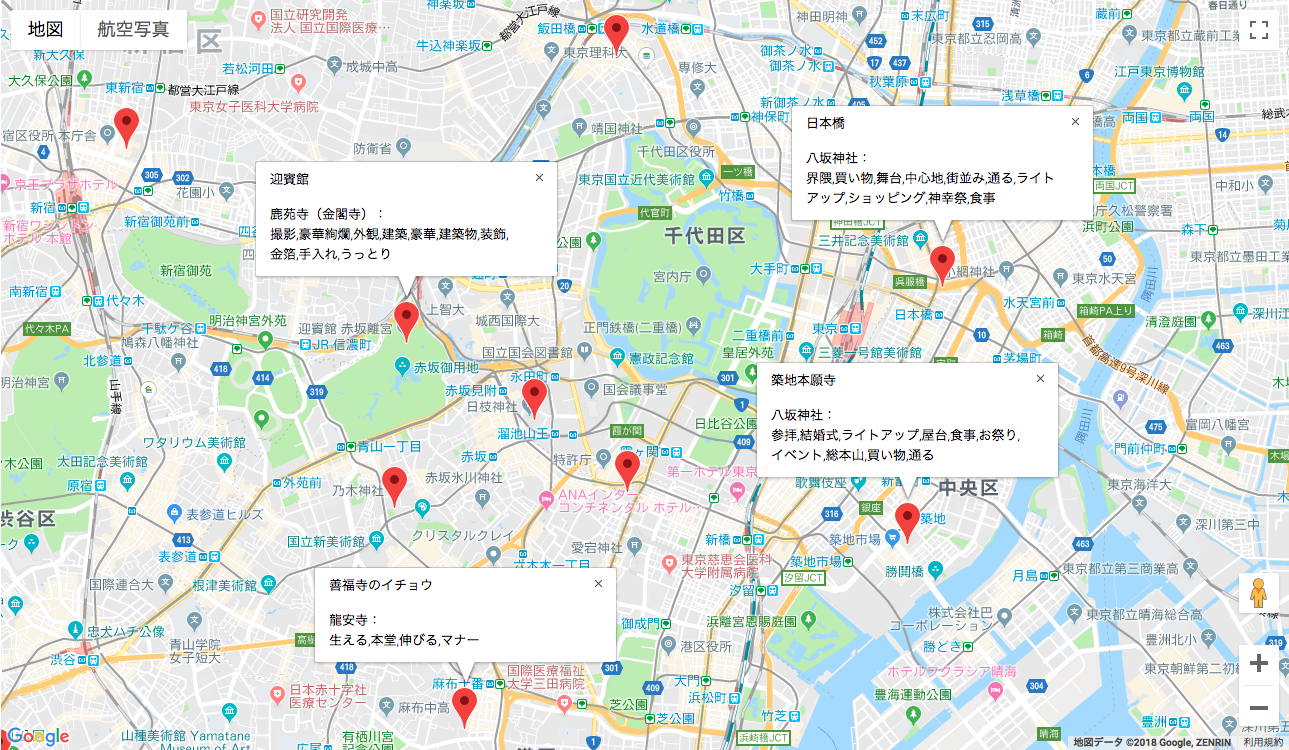
\includegraphics[clip,width=8.5cm,bb=0 0 1289 750]{picture/Photo_Map.png}
    \caption{User interface of prototype system}
    \label{fig:photo_map}
   \end{center}
\end{figure}

\subsection{Example of explained unfamiliar spots}
\label{subsec:Example of explained unfamiliar spots}

\begin{table}[t]
  \caption{The set of Familiar spot and Unfamiliar spot}
  \label{table:Familiar spot group and Unfamiliar spot group}
  \centering
  \begin{tabular}{l|l}
  \hline
  \multicolumn{1}{c|}{Familiar Spot Name} & \multicolumn{1}{c}{Unfamiliar Spot Name} \\ \hline
  Sensoji Temple                          & Tokyo Disneyland (R)                     \\
  Odawara-jo Park                         & Shinjuku Gyoen                           \\
  Fushimiinari-taisha Shrine              & Tokyo Skytree                            \\
  Nara Park                               & Tokyo Tower Main Deck            \\
  Mishima Skywalk                         & Meiji Jingu                              \\ \hline
  \end{tabular}
\end{table}

\begin{table*}[t]
  \caption{Explanation information}
  \label{table:Explanation information}
  \centering
  \begin{tabular}{l|l|l}
  \hline
  \multicolumn{1}{c|}{Unfamiliar Spot} & \multicolumn{1}{c|}{Familiar Spot} & \multicolumn{1}{c}{Explanation Information}                     \\ \hline
  Shinjuku Gyoen                      & Odawara-jo Park                         & flower viewing, bloom, inside the park, cherry-blossoms, leisurely, maintenance, nature, play equipment, azalea          \\
  Tokyo Skytree                     & Mishima Skywalk                    & Mt. Fuji, swing, high fear, ceiling, magnificent view, elevator, panorama, observation deck, rising
 \\ \hline
  \end{tabular}
\end{table*}

Table \ref{table:Familiar spot group and Unfamiliar spot group} shows an example of a set of user's familiar spots and unfamiliar spots.
Unfamiliar spots are five spots randomly selected from within Tokyo.
Table \ref{table:Explanation information} shows the results of explainable words using the proposed method in Section \ref{sec:An Explainaton Method of Unfamiliar Tourist Spots}.

Focusing on the feature of the park, it is thought that the spot closest to the park in the set of unfamiliar spots is ``Shinjuku Gyoen''.
In the set of familiar spots there are two parks, ``Odawara-jo Park'' and ``Nara Park''.
``Odawara-jo Park'' has a lot of descriptions about flowers and play equipments, on the other hand, ``Nara Park'' has a lot of descriptions about deers and grass.
Because ``Shinjuku Gyoen'' has a lot of descriptions about flowers and play equipments, it seems to be related to ``Odawara-jo Park''.

``Mishima Skywalk'' is considered to be a feature with a good view and high in the set of familiar spots.
On the other hand, ``Tokyo Skytree'' and ``Tokyo Tower Main Deck'' are the scenes with a good view and high in the set of unfamiliar spots.
In this case, we think both are correct answers. In this example, it was associated with ``Tokyo Skytree'' which is considered to have better view.
Also, ``Mt. Fuji'' is extracted as an explainable keyword. It is common as a word that emphasizes the good view and it seems that it expresses the relationship appropriately.
The proposed method can show the feature of each relationship.

\section{Evaluation Experiment}
\label{sec:Evaluation Experiment}
\subsection{Settings of experiment}
\label{subsec:Settings of experiment}
We evaluate proposed method by comparing with other method.
We compare following three methods.
\begin{description}
\item[A]Metadata (category, duration time, season)
\item[B]Paragraph vector (feature vector)
\item[C]Proposed Method (relative feature vector)
\end{description}

The method A is metadata used for searching spots on the sightseeing spots search site.
We selected three metadata that are often used for search as follows.
\begin{itemize}
\item category: e.g.) Shrine / Temple,Tourist facilities / Tourist tours etc.
\item duration time: e.g.) less than 1 hour,1 to 2 hour etc.
\item season: e.g.) 1 to 12 month, spring, summer, autumn, winnter
\end{itemize}

In method A, familiar spot and unfamiliar spot of the same category, same duration time, same season are extracted. If it can not be extracted, delete the conditions in order of season, duration time, category.
If there are multiple unfamiliar spots, we select the one with the largest number of reviews.
Finally, we extract the explainable words using section \ref{subsec:Extraction of explainable words for role} and present them to the subjects.

The method B use the feature of each spot using the feature vector created in section \ref{subsec:Generating feature vector using user reviews of spot}.
And, we extract the explainable words using section \ref{subsec:Extraction of explainable words for role} and present them to the subjects.

We collected 24 subjects using CrowdWorks\footnote{CrowdWorks is a crowdsourcing service in Japan. https://crowdworks.jp/}.
We presented explainable information of unfamiliar spots based on subjects' familiar spots using each method.
First, the subject inputted tourist spots that he/she had already visited and he/she likes. The number of spots to be input by the subject is four to ten.
In this experiment, in order to match the input character string with the spot name in the system, the subject selected from the spot name candidates similar to the input character string.
Next, the subjects never went on a trip etc and entered prefectures / areas that we would like to visit.
We presented familiar and unfamiliar spots associated with methods A to C and their explainable keywords.
We presented up to five keywords (N = 5).
Subjects evaluated the results by choosing one out of the following five options.
\begin{enumerate}
  \item No keyword.
  \item There is a relationship between the two spots, and the relationship became clear by keywords.
  \item There is a relationship between the two spots, and I noticed the relationship for the first time by keyword.
  \item There is a relationship between the two spots, but the keyword does not represent the relation.
  \item There is no relationship between the two spots.
\end{enumerate}

\subsection{Result}
\label{subsec:Result}

\begin{table}[t]
  \caption{Experimental results}
  \label{table:Statistics on the number of data of experiment results}
  \centering
  \begin{tabular}{c|r|r|r|r}
  \hline
  Evaluation & \multicolumn{1}{c|}{Method A} & \multicolumn{1}{c|}{Method B} & \multicolumn{1}{c|}{Method C} &  \multicolumn{1}{c}{Total} \\ \hline
  1  & 0                      & 0                      & 0                      & 4                      \\
  2  & 19                     & 44                     & 32                     & 121                    \\
  3  & 20                     & 62                     & 53                     & 191                    \\
  4  & 1                      & 3                      & 3                      & 10                     \\
  5  & 6                      & 21                     & 21                     & 68                     \\ \hline
  Total & 46                     & 130                    & 109                    & 285                    \\ \hline
  \end{tabular}
\end{table}

Table \ref{table:Statistics on the number of data of experiment results} shows the number of each experimental result of method A to C.
In the evaluation experiment, the total of usable data is 285.
The method A has the smallest number of familiar spots associated with unfamiliar spots.
The method B has the largest number of familiar spots related to unfamiliar spots.

\begin{table}[t]
  \caption{Percentage of evaluation in explanation information}
  \label{table:Percentage of evaluation in explanation information}
  \centering
  \begin{tabular}{c|r|r|r}
  \hline
  Evaluation & \multicolumn{1}{c|}{Method A} & \multicolumn{1}{c|}{Method B} & \multicolumn{1}{c}{Method C} \\ \hline
  1  & 0.00\%                     & 0.00\%                     & 0.00\%                                         \\
  2  & 41.30\%                    & 33.85\%                    & 29.36\%                                       \\
  3  & 43.48\%                    & 47.69\%                    & 48.62\%                                       \\
  4  & 2.17\%                     & 2.31\%                     & 2.75\%                                         \\
  5  & 13.04\%                    & 16.15\%                    & 19.27\%                                       \\ \hline
  \end{tabular}
\end{table}

\begin{table*}[t]
  \caption{When the categories of the familiar spots are different or  percentage of evaluation when similar}
  \label{table:When the categories different or similar}
  \centering
  \begin{tabular}{c|r|r}
  \hline
  & \multicolumn{1}{c|}{\begin{tabular}[c]{@{}c@{}}When the familiar spots are different\end{tabular}} & \multicolumn{1}{c}{\begin{tabular}[c]{@{}c@{}}When the familiar spots are similar\end{tabular}} \\ \hline
  Method B \& Option 2 & 56.82\%                            & 43.18\%                            \\
  Method C \& Option 2 & 71.87\%                            & 28.13\%                            \\ \hline
  Method B \& Option 3 & 51.61\%                            & 48.39\%                            \\
  Method C \& Option 3 & 52.83\%                            & 47.170\%                            \\ \hline
\end{tabular}
\end{table*}

Table \ref{table:Percentage of evaluation in explanation information} shows the ratio of the number of the experimental results as the option 1 to 5 in the method A to C.
Many subjects choose option No.2 for Method A. From this, it can be seen that the method A can associate spots having apparent relationships.
Compared to the other methods, in Method C (proposed method), the ratio of No.2 option decreases and the ratio of No.3 option increases. From this, we think that method C finds and presents hidden relationships. However, as the ratio of option No. 5 also increases, we can say that it is easier to extract irrelevant spots.

When option 2 and option 3 are summed, method A is the highest. From this, we can say that the accuracy of the association of spots for explanation is the highest. However, as described above, the meaning of option 2 is a natural relationship, and Method A can extract only a small number.
For us, options 2 and 3 are observed to be in a trade-off relationship. Option 2 is a relationship which does not need to explain botherly, option 3 is a relationship worthy of explanation.
We think that it is important to increase choice 3 as much as possible while maintaining option 2. From this point of view, it is considered that Method B and the proposed method show the same degree of accuracy.

Option 3 has a high possibility of changing to option 5 if keyword extraction fails. Therefore, we need to improve the method of keyword extraction.

For method B and method C, the case where the category of the familiar spot inputted by the subject is different is similar to the case where the categories of the familiar spots input by the subject are different, the ratio of the evaluation of the option 2 and the option 3 is the table \ref{table:When the categories different or similar}.
Using method C, which is the proposed method, subjects can present meaningful keywords without relation to a certain spot that the subject has familiar visited.
By using the relative feature vector, it can be said that the characteristics of each spot can be found over the category.
In the case where the genres of the familiar spots are similar, the method B is better than the case.

\section{Conclusions and Future Work}
\label{sec:Conclusions and Future Work}
We focused on the difficulty of understanding the tourist spots searched by using the tourist spot search engine in ranking, recommendation information, categories, and so on., if the presented tourist spots are unfamiliar for the user.
In order to support understanding of unfamiliar spots, we proposed an explanatory method to support understanding by comparing unfamiliar spots with familiar spots that users have already visited.

In the evaluation experiment, we evaluate four method of explanatory information.
As a result, in the case of using categories, the number of familiar spots associated with unfamiliar spots is the smallest.
By using the relative feature vector and harmonic mean, the characteristics of each spot can be obtained.
In addition, we confirmed that it was possible to correlate unexpected unfamiliar spots with familiar spots, and that there is a possibility that interest and attention can be drawn to tourist spots that users do not know.

As future works, we analyze experimental result such as the relevance between keywords presented to users.
We also plan to evaluate the effectiveness and relevance of each keyword presented to the user.

\section*{Acknowledgment}
This work was supported by ISPS KAKENHI of Grant-in-Aid for Scientific Research(C) Grant Number 18K11551.

\ifCLASSOPTIONcaptionsoff
  \newpage
\fi

\begin{thebibliography}{1}
  \bibitem{Codd01}
    T. Kurashima, T. Iwata, G. Irie and K. Fujimura.,
      ``Travel route recommendation using geotags in photo sharing sites'',
      CIKM '10 Proceedings of the 19th ACM international conference on Information and knowledge management, pp.579-588, 2010
  \bibitem{Codd02}
    R. Kitamura and T. Itoh,
      ``Tourist Spot Recommmendation Applying Generic Object Recognition with Travel Photos'',
      ITE Tech. Rep., Vol.42, No.12, AIT2018-94, pp.185-188, 2018
  \bibitem{Codd03}
    A. J. Cheng, Y. Y. Chen, Y. T. Huang and Winston H. Hsu,
      ``Personalized Travel Recommendation by Mining People Attributes from Community-Contributed Photos'',
      MM '11 Proceedings of the 19th ACM international conference on Multimedia, pp.83-92, 2011
  \bibitem{Codd04}
    K. J. Holyoak and P. Thagard,
      ``Mental Leaps: Analogy in Creative Thought, MIT Press'',
      Journal of Japanese Society for Artificial Intelligence,  Vol.11, No.3,  pp.489, 1996
  \bibitem{Codd05}
    D. Gentner,
      ``Structure-Mapping: A Theoretical Framework for Analogy'',
      Cognitive Science, Vol.7, pp.155-170, 1983
  \bibitem{Codd06}
    M. L. Gick and K. J. Holyoak,
      ``Analogical Problem Solving'',
      Cognitive Psychology, Vol.12, pp.306-355, 1980
  \bibitem{Codd07}
    M. L. Gick and K. J. Holyoak,
      ``Scheme Induction and Similarity in Analogical Transfer'',
      Cognitive Psychology, Vol.15, pp.1-38, 1983
  \bibitem{Codd08}
    Z. Chen and M. W. Daehler,
      ``Positive and Negative Transfer in Analogical Problem-solving by 6-years-old Children'',
      Cognitive Development, Vol.4, No.4, pp.327-344, 1989
  \bibitem{Codd09}
    K. J. Holyoak and P. Thagard,
      ``Analogical Mapping by Constraint Satisfaction'',
      Cognitive Science, Vol.13, pp.295-355, 1989
  \bibitem{Codd10}
    Quoc V. Le and Tomas Mikolov,
      ``Distributed representations of sentences and documents'',
      In Proceedings of the 31th International Conference on Machine Learning, ICML 2014, pp. 1188-1196, 2014
  \bibitem{Codd11}
    T. Kudo, K. Yamamoto and Y. Matsumoto,
    ``Applying Conditional Random Fields to Japanese Morphological Analysis'',
    Proceedings of the 2004 Conference on Empirical Methods in Natural Language Processing (EMNLP-2004), pp.230-237, 2004

\end{thebibliography}
\end{document}
